\section{Graph Search Planners} \label{A. Graph search planners}
The discussed algorithms from this section represent a classic solution to the path finding problem. The majority of them require the world map to be represented as a graph or grid \cite{choset2005principles}.

A graph (See Figure \ref{fig:graphs}) is a data structure that is composed of nodes (vertices) and edges usually represented as $G = (V, E)$ where $V$ is a collection of nodes (vertices) and $E$ is a collection of edges. The edges can be undirected (undirected graph; bidirectional movement) or directed (directed graph; unidirectional movement). Each edge can have an associated weight (weighted graph) or not (unweighted graph), which might represent the movement cost between two nodes \cite{choset2005principles}.

\begin{figure}[h!]
  \centering
  \begin{subfigure}[b]{0.18\linewidth}
    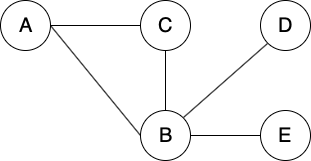
\includegraphics[width=\linewidth]{images/undirected_unweighted_graph.png}
     \caption{Undirected unweighted graph}
  \end{subfigure}
  \hfill
  \begin{subfigure}[b]{0.18\linewidth}
    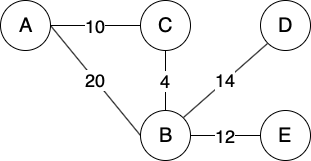
\includegraphics[width=\linewidth]{images/undirected_weighted_graph.png}
    \caption{Undirected weighted graph}
  \end{subfigure}
  \hfill
  \begin{subfigure}[b]{0.18\linewidth}
    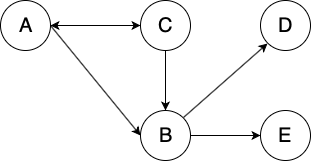
\includegraphics[width=\linewidth]{images/directed_unweighted_graph.png}
    \caption{Directed unweighted graph}
  \end{subfigure}
  \hfill
  \begin{subfigure}[b]{0.18\linewidth}
    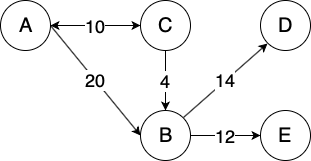
\includegraphics[width=\linewidth]{images/directed_weighted_graph.png}
    \caption{Directed weighted graph}
  \end{subfigure}
  \caption{Graph examples. The nodes are represented with a circle, and the identifier is the letter inside them. The edges are represented by lines or arrows, and the values from them represent weight values}
  \label{fig:graphs}
\end{figure}

A grid (See Figure \ref{fig:grids}) is a two-dimensional table that allows movement to nearby cells. This data structure can be easily translated to an undirected unweighted graph where grid cells represent nodes and neighbours represent undirected edges. The neighbours are defined in terms of the grid connectivity type which can be 4-point connectivity (up, down, left, right) or 8-point connectivity (all 4-point connectivity neighbours, principal diagonal and secondary diagonal) \cite{choset2005principles}. We are going to assume 8-point connectivity for all grids unless explicitly stated.

\begin{figure}[h!]
  \centering
  \begin{subfigure}[b]{0.18\linewidth}
    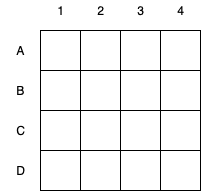
\includegraphics[width=\linewidth]{images/4x4_grid.png}
     \caption{4$\times$4 normal grid\newline\newline}
  \end{subfigure}
  \hfill
  \begin{subfigure}[b]{0.18\linewidth}
    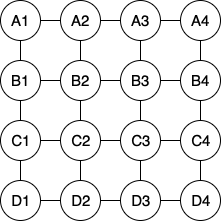
\includegraphics[width=\linewidth]{images/4_way_graph.png}
    \caption{4-point connectivity graph representation}
  \end{subfigure}
  \hfill
  \begin{subfigure}[b]{0.18\linewidth}
    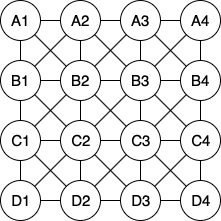
\includegraphics[width=\linewidth]{images/8_way_graph.png}
    \caption{8-point connectivity graph representation}
  \end{subfigure}
  \caption{4x4 grid example with associated 4-point and 8-point connectivity graphs. In 4-point connectivity, the neighbours are up, down, left and right. In 8-point connectivity, the neighbours are all 4-point connectivity neighbours, the principal diagonal and the secondary diagonal. The numbers at the top and left of the grid represent coordinates}
  \label{fig:grids}
\end{figure}

A tree (See Figure \ref{fig:trees}) is a directed graph with a root (i.e. a node that has no incoming edges) where each node has directed edges to their children. A particular property of the tree is that it contains no cycles. This data structure is essential as most algorithms have to walk the graph in some way (depth-first search, breadth-first search) in order to discover a possible path. Depth-first search (DFS) \cite{Cormen:2009:IAT:1614191} is a graph walking method that can be implemented using a stack (Last In First Out (LIFO) data structure) or recursion (stack is preferred, due to the recursion depth constraint that most programming languages incorporate). DFS starts by “expanding” the root (i.e. visit the node and push the node’s children onto the stack) and then iteratively expands the latest node from the stack. Thus, we initially visit the first children of the node we expand and then visit its children recursively before continuing with the second child. Breadth-first search (BFS) \cite{Cormen:2009:IAT:1614191} is another graph walking method that uses a queue (First In First Out FIFO data structure). BFS starts by expanding the root and then it repeats the process iteratively for the children. Thus we first visit \textbf{all} of the children of the node we expand and then we continue to expand each child. When BFS has to expand a node, it chooses the one in the front of the queue, and then it puts \textbf{all} of the children at the end of the queue. The result of both methods is a tree \cite{choset2005principles}.

\begin{figure}[h!]
  \centering
  \begin{subfigure}[b]{0.18\linewidth}
    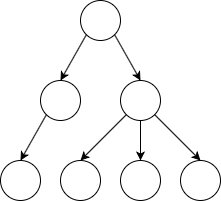
\includegraphics[width=\linewidth]{images/tree_example.png}
     \caption{A tree}
  \end{subfigure}
  \hfill
  \begin{subfigure}[b]{0.18\linewidth}
    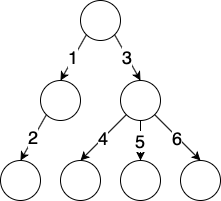
\includegraphics[width=\linewidth]{images/dfs.png}
    \caption{DFS walk}
  \end{subfigure}
  \hfill
  \begin{subfigure}[b]{0.18\linewidth}
    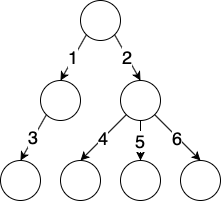
\includegraphics[width=\linewidth]{images/bfs.png}
    \caption{BFS walk}
  \end{subfigure}
  \caption{An example of a tree along with a DFS and BFS walk. The numbers indicate the order of expansions}
  \label{fig:trees}
\end{figure}

The worst case time complexity of DFS is $\mathcal{O}(b^d)$ and the worst case space complexity is $\mathcal{O}(b \cdot d)$ if a stack is used and $\mathcal{O}(d)$ if recursion is used, where $b$ is the branching factor (the average number of a node's children) and $d$ is the visiting depth. Time complexity is trivial as at each step we run a new search for all the node children $b$, and we do this $d$ times. If we use a stack, for each node, we push all children onto the stack. We do this $d$ times, and each node has $b$ children. Therefore the space complexity is $\mathcal{O}(b \cdot d)$. When using recursion, the space complexity is lower as it is defined in terms of the recursion depth (we do not use all children at once at each recursion step). However, we still prefer to use the stack in practice, due to the programming language limitations \cite{Cormen:2009:IAT:1614191}.

The worst case time and space complexity of BFS is $\mathcal{O}(b^d)$. The time complexity follows the same reasoning as DFS. Space complexity is given by the number of nodes in the queue at one time which is equal to the number of the nodes on each layer of the tree which is $\mathcal{O}(b^d)$ as each layer node count grows exponentially \cite{Cormen:2009:IAT:1614191}.

When talking about complexities we have opted for the $b$ (branching factor) and $d$ (depth) notation instead of the $|E|$ (number of edges) and $|V|$ (number of vertices/nodes) (e.g. DFS space complexity is the same as BFS space complexity $\mathcal{O}(|V|)$). We are going to discuss algorithms which attempt to prune the search space, and we can infer more information from the first notation rather than the second one \cite{Cormen:2009:IAT:1614191}.

In practice, we prefer to use BFS when dealing with problems that attempt to find an optimal solution (due to the visiting pattern) and DFS when we want to visit the whole tree without caring about the visiting pattern or when we have memory constraints.

\subsection{Wave-front Planner} \label{sec: wave-front}
The Wave-front Planner algorithm \cite{choset2005principles, luo2014effective} (See Figure \ref{fig:wave_front_planner}) is one of the simplest solutions to the pathfinding problem. The algorithm can only run on grids (two dimensional or higher). The main idea is to have a separate grid with initial values of 0 then "propagate" a wave from the goal position to the agent position. Thus, we essentially create a potential function on the grid. 

The wave is propagated by applying BFS to the separate grid from the goal position and then labelling the nodes on the same level of the tree with the level number. Thus, we first visit all the (valid) neighbours of the goal and mark the positions on the new grid with a 2 (as the goal position is marked with 1). Then we repeat the process for the nodes labelled with a 2 by expanding them and marking their \textbf{not visited} neighbours with a 3. The process is repeated until we hit the agent position. After that, we apply gradient descent from the agent position to the goal position. We start from the agent marked with number $x$ and then search its neighbours for a node marked with $x-1$. If there are multiple choices we can choose a random number as the invariant of the algorithm states that, given any node, the distance between itself and the agent is the absolute difference between their grid values (See Algorithm \ref{alg: wave_front_planner}).

% figures align
\vspace{-0.5cm}
$$dist(n) = abs(grid(G) - grid(n))$$
\vspace{-0.5cm}

We can easily prove that the algorithm finds the optimal solution in terms of minimum distance as we have used BFS to expand the nodes. If we would have used DFS instead, we could have still found a solution, but it would not necessarily be optimal due to the visiting pattern in DFS. The path might not be optimal in environments where the edge transition cost is not equal in all directions (e.g. moving on the diagonal ($\sqrt{2}$) is more expensive than moving vertically or horizontally (1) based on the Euclidean distance).

The worst case time and space complexity are given by the visiting method (BFS in our case) which is $\mathcal{O}(b^d)$, where $b$ is the branching factor, and $d$ is the depth of the solution (\textit{Get-Backtrace} is $\mathcal{O}(d)$).

One of the major drawbacks to this approach is that the optimal path is dangerously close to the obstacles (as only the attraction function is used) and in the real world, it might lead to collisions. It is also computationally expensive as the planner's search space is quite large since it does not apply any pruning. Moreover, the time and space complexity increase exponentially with the dimension of the environment. In a 2D grid with 8-point connectivity $b$ is 8, but in a 3D grid world $b$ is $3 \times 9 - 1 = 26$ (we subtract the (0, 0, 0) direction), where $b$ is the branching factor. A nice way to visualise the increase of $b$ is to count the number of combinations on each direction. Each coordinate has 3 configurations (1, 0, -1) and the number of combinations is given by $3^D$, where $D$ is the dimension. Therefore, $b = 3^D - 1$ (we have to subtract the (0, 0, ..., 0) configuration as it is not a valid neighbour). Therefore, time and space complexity becomes $\mathcal{O}((3^D)^d)$. However, because we are working with real-world robots, we can only consider 2D and 3D environments (2D for ground robot, 3D for drones and flying robots).

% A possible memory optimisation is to use the same input grid if the grid entities are labelled with a number (0 clear, 1 wall, -1 agent, 2 goal). However one requirement is that the goal has to be identified with a number higher then all other available entities.

\begin{figure}[]
  \centering
  \begin{subfigure}[b]{0.2\linewidth}
    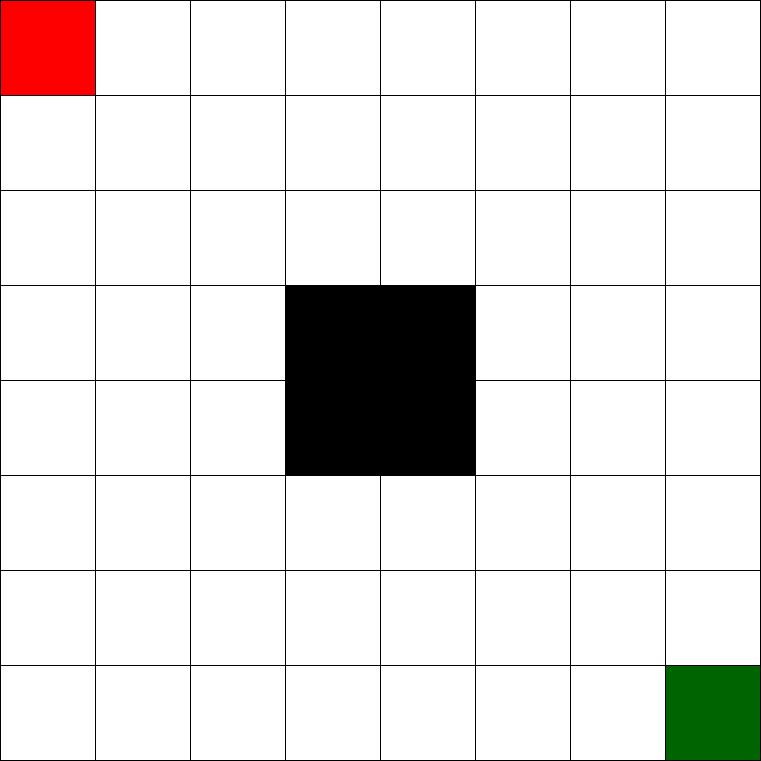
\includegraphics[width=\linewidth]{images/simple_grid.png}
     \caption{Starting 8x8 grid}
  \end{subfigure}
  \hfill
  \begin{subfigure}[b]{0.2\linewidth}
    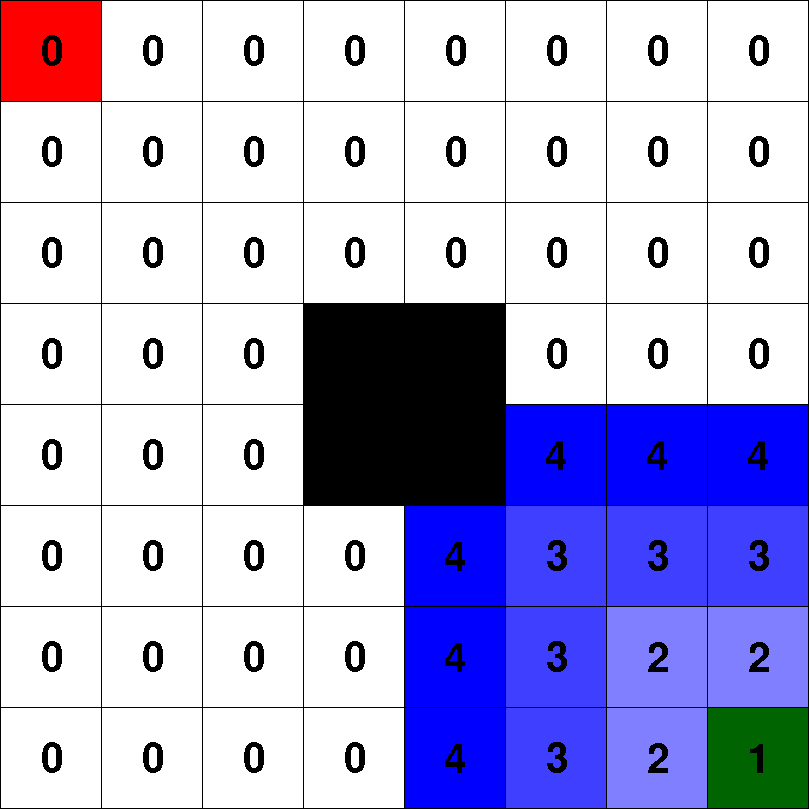
\includegraphics[width=\linewidth]{images/wave_front_planner_1.png}
     \caption{Iteration 1}
  \end{subfigure}
  \hfill
  \begin{subfigure}[b]{0.2\linewidth}
    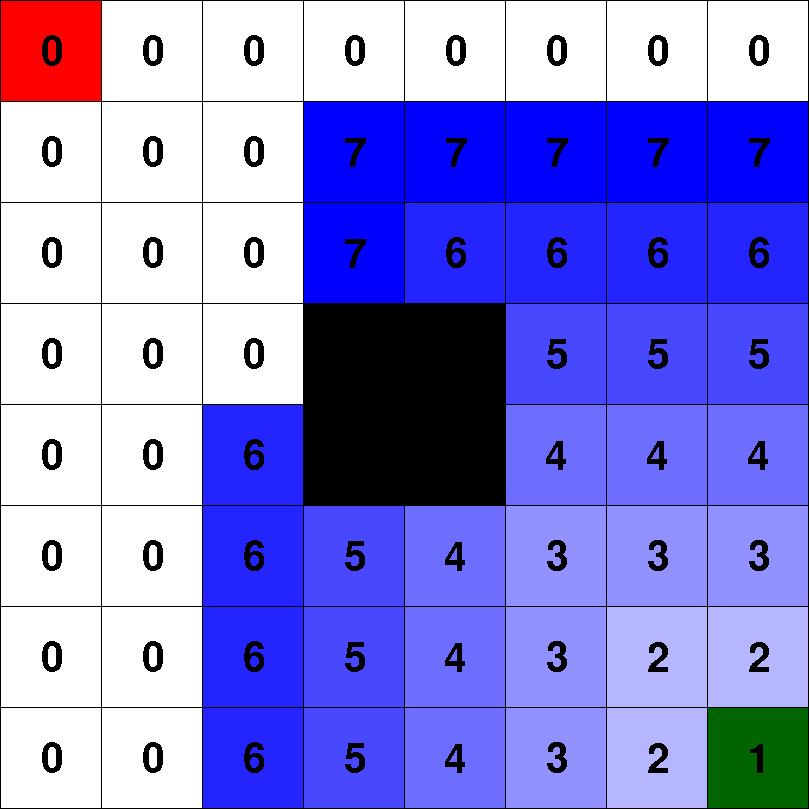
\includegraphics[width=\linewidth]{images/wave_front_planner_2.png}
    \caption{Iteration 2}
  \end{subfigure}
  \hfill
  \begin{subfigure}[b]{0.2\linewidth}
    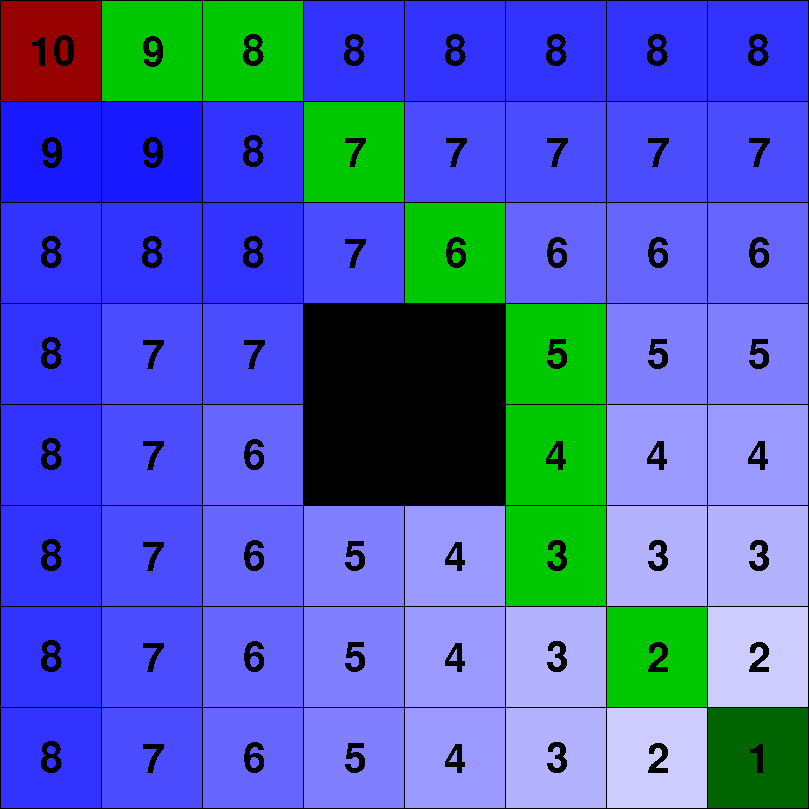
\includegraphics[width=\linewidth]{images/wave_front_planner_3.png}
    \caption{Final trace}
  \end{subfigure}
  \caption{Wave-front Planner algorithm run on an 8x8 grid (4 iteration points shown: start, 1, 2, final trace). The red square represents the agent start position, the dark green square represents the goal position, black squares represent obstacles, white squares represent the clear path, light green squares represent the final path chosen by the algorithm. The numbers in each grid cell represent the gradient map and the white (min) - dark blue (max) gradient colour is another representation of the gradient map}
  \label{fig:wave_front_planner}
\end{figure}

\begin{algorithm}[h!]
\caption{Wave-Front Planner}
\label{alg: wave_front_planner}
\begin{algorithmic}[1]

\Procedure{Get-Backtrace}{$step\_grid$, $M\colon(A, Os, G)$}
    \State $trace \gets [A]$
    % \State
    \While {$current$ is not $A$}
        \State $current \gets \forall n \in Neighbours(current). step\_grid[n] = step\_grid[current] - 1$
        \State add $current$ to $trace$
    \EndWhile
    % \State
    \State \Return $trace$
\EndProcedure
\\
    
\Procedure{Wave-Front-Planner}{$M\colon(A, Os, G)$}
    \State Initialize queue $q$ with (1, $G$)
    \State Initialize $step\_grid$ as array with same size as map
    \State $visited \gets \{\}$
    \State
    \Repeat
        \State ($current\_count$, $current\_node$) $\gets$ pop front $q$
        \State add $current\_node$ to $visited$
        \State $step\_grid[current\_node]$ $\gets$ $current\_count$
        \State
        \If {$current\_node$ is $A$}
            \State follow $\textit{Get-Backtrace}(step\_grid, M)$
            \State \Return 
        \EndIf
        \State
        \For {\textbf{each} $neighbour$ in $Neighbours(current\_node)$}
            \If {$neighbour$ is not in $visited$}
                \State append ($current\_count$ + 1, $neighbour$) to $q$
            \EndIf
        \EndFor
    \Until $q$ is empty
    \State
    \State goal was not found
\EndProcedure
\end{algorithmic}
\end{algorithm}

\subsection{A*} \label{sec:a_star}
The A* algorithm \cite{choset2005principles, duchovn2014path, zhang2014multiple, 5937169} (See figures \ref{fig:a_star}, \ref{fig:a_star_expansion}) is mostly designed to run on weighted graphs, but can be adapted to run on grids as well if we convert the grid to a graph with weights based on the Euclidean distance (1 for vertical/horizontal movement and $\sqrt{2}$ for diagonal movement).

The difference between A* and Wave-front Planner is that A* aims to prune the search space by using a heuristic function $h$ which is usually the Euclidean distance (8-point connectivity) or the Manhattan distance (4-point connectivity) (See Figure \ref{fig:distances}).

\begin{figure}[h!]
  \centering
  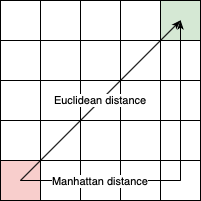
\includegraphics[scale=0.5]{images/distances.png}
  \caption{Euclidean and Manhattan distances. Red square is agent and green square is goal}
  \label{fig:distances}
\end{figure}

It is implemented using a priority queue in which the priorities are a function $f(n) = g(n) + h(n)$, where $h$ is the heuristic function mentioned above and $g$ is a function which represents the total actual distance travelled from the agent to the node $n$. The cost function $c(x, y)$ returns the graph weight cost from node $x$ to node $y$ ($x$ and $y$ have to be connected). The algorithm starts with the agent node in the priority queue. Then, the element with the highest priority (i.e. lowest $f(n)$) is picked and expanded, and its children are inserted into the priority queue. Each child will have a parent $p$, which will help us trace back the path at the end. When we expand a child we set $p(child) = n$. If a path is found, we update the goal parent. We stop the process only when the priority queue is empty or when the next priority is less than or equal to the optimal distance found. All expanded nodes are marked as seen, so we do not have to revisit them. When we expand a node, if any of its children are already in the queue we add them again if the path through the current node gives a higher priority ($g(n) < g(child)$) and update the child's parent ($p(child) = n, g(child) = g(n) + c(n, child)$). It does not matter if we add the children again to the queue as we know that $f_{cur}(child) < f_{old}(child)$ so we will visit the higher priority option first. When we stop, we compute the trace by recursively looking at the next parent from the goal until we find the agent (See Figure \ref{fig:a_star_expansion}, Algorithm \ref{alg: a_star}).

A* finds the shortest path, if and only if, the heuristic function is optimistic. An optimistic heuristic function is always less than or equal to the shortest distance.

The worst case time and space complexity of A* is $\mathcal{O}(b^d)$, where $b$ is the branching factor, and $d$ is the depth of the solution because the underlying algorithm structure is similar to BFS (\textit{Get-Backtrace} is $\mathcal{O}(d)$). However, by using a good heuristic function, the time and space complexity becomes $\mathcal{O}(\hat{b}^d)$ where $\hat{b}$ is the reduced branching factor (i.e. A* prunes the search).

% \todo{Cite wikipedia and stackoverflow??}
% https://en.wikipedia.org/wiki/A*_search_algorithm
% https://cs.stackexchange.com/questions/56176/a-graph-search-time-complexity

The significant advantage of A* is that the search space is pruned quite a lot, but it still shares the same issue as the other graph search planners: the search space grows exponentially with the grid dimension.

One of the major drawbacks is that it is not trivial to find a proper heuristic function for some environments (e.g. maps that do not define a metric space such as networks). In general, the Euclidean distance or the Manhattan distance are good choices for the heuristic function. Lastly, A* is an offline method (the internal state of the algorithm cannot be externally modified) meaning that external updates to the map are forbidden. Therefore, offline algorithms such as A* do not support dynamic and partial knowledge environments.

\pagebreak

\begin{figure}[h!]
  \centering
  \begin{subfigure}[b]{0.2\linewidth}
    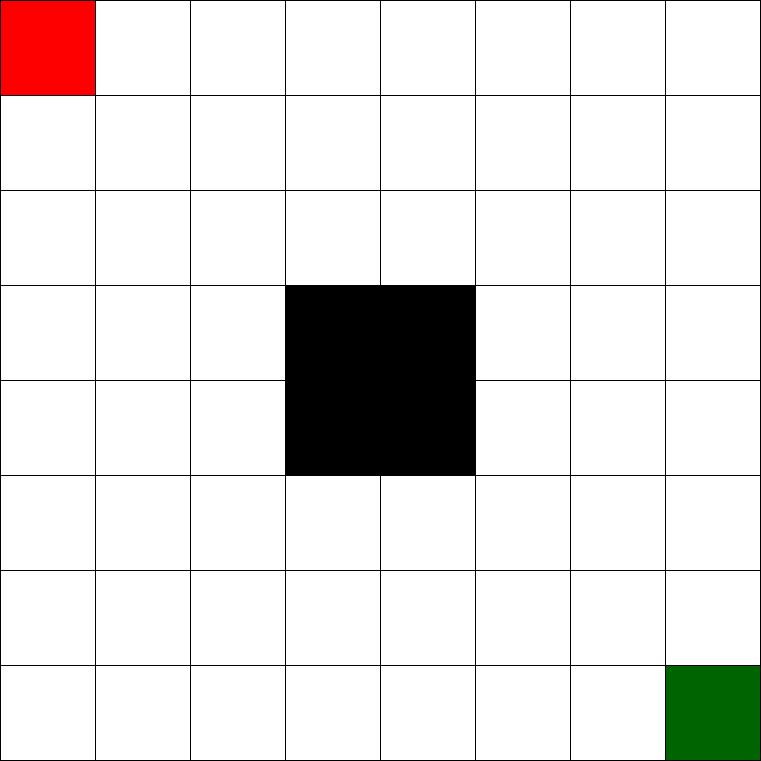
\includegraphics[width=\linewidth]{images/simple_grid.png}
     \caption{Starting 8x8 grid}
  \end{subfigure}
  \hfill
  \begin{subfigure}[b]{0.2\linewidth}
    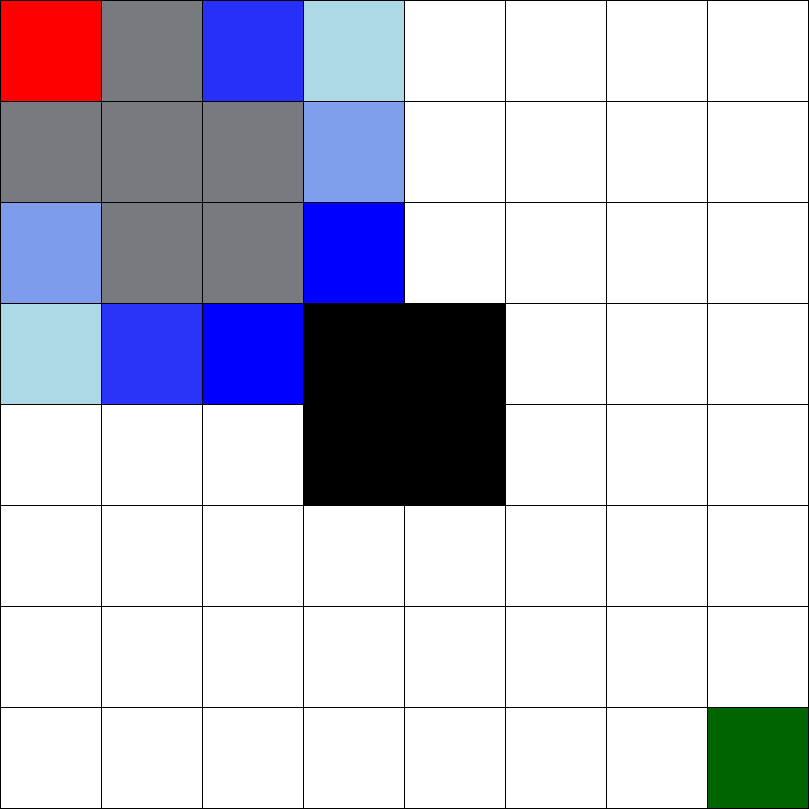
\includegraphics[width=\linewidth]{images/a_star_1.png}
     \caption{Iteration 1}
  \end{subfigure}
  \hfill
  \begin{subfigure}[b]{0.2\linewidth}
    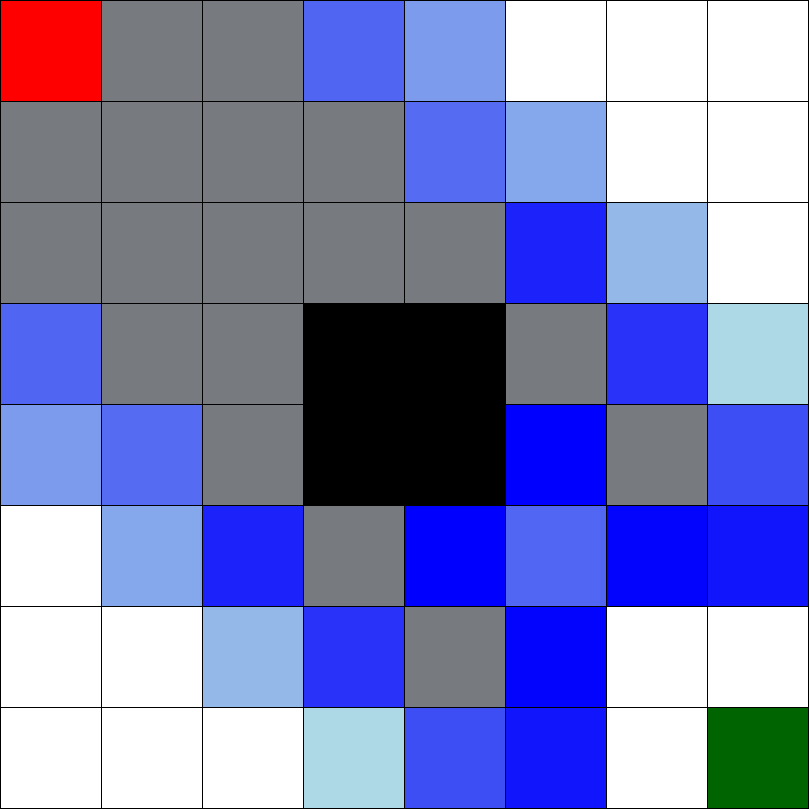
\includegraphics[width=\linewidth]{images/a_star_2.png}
    \caption{Iteration 2}
  \end{subfigure}
  \hfill
  \begin{subfigure}[b]{0.2\linewidth}
    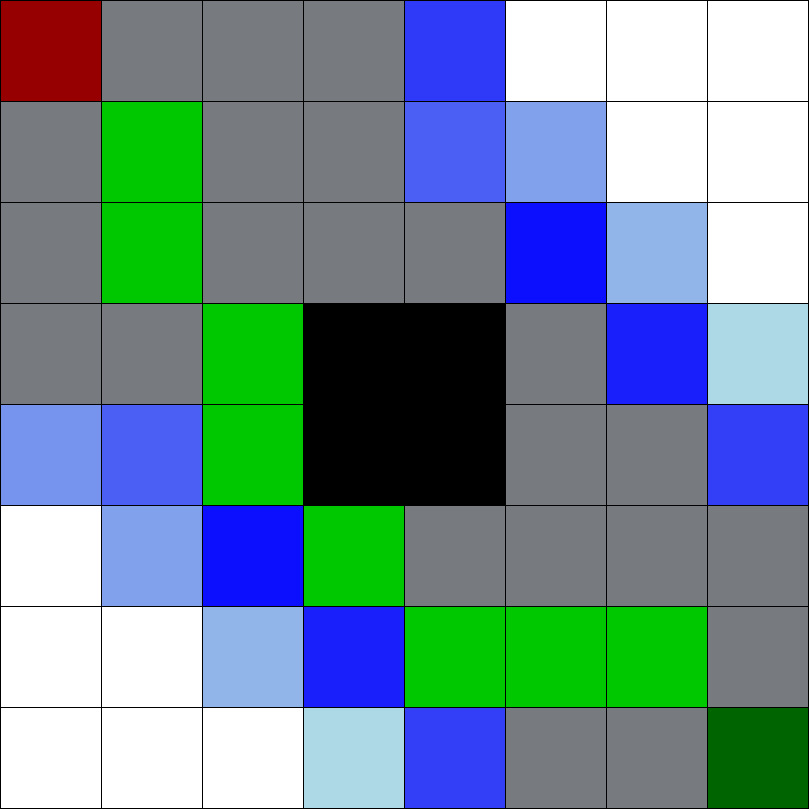
\includegraphics[width=\linewidth]{images/a_star_3.png}
    \caption{Final trace}
  \end{subfigure}
  \caption{A* algorithm run on an 8$\times$8 grid (4 iteration points shown: start, 1, 2, final trace). The red square represents agent start position, the dark green square represents the goal position, black squares represent obstacles, white squares represent the clear path, light green squares represent the final path chosen by the algorithm. The dark grey squares represent the visited set, and the blue squares represent the priority queue (the darker the blue, the higher the priority)}
  \label{fig:a_star}
\end{figure}

\begin{figure}[h!]
  \centering
  \begin{subfigure}[b]{0.2\linewidth}
    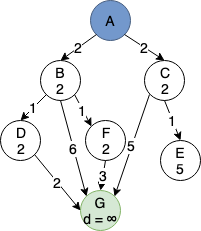
\includegraphics[width=\linewidth]{images/a_star_expansion1.png}
     \caption{Iteration 1}
  \end{subfigure}
  \hfill
  \begin{subfigure}[b]{0.2\linewidth}
    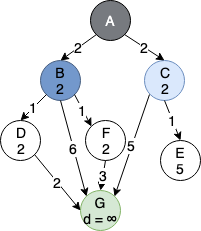
\includegraphics[width=\linewidth]{images/a_star_expansion2.png}
     \caption{Iteration 2}
  \end{subfigure}
  \hfill
  \begin{subfigure}[b]{0.2\linewidth}
    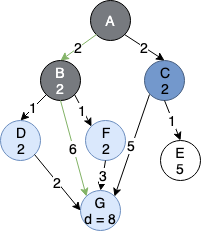
\includegraphics[width=\linewidth]{images/a_star_expansion3.png}
    \caption{Iteration 3}
  \end{subfigure}
  \newline
  \begin{subfigure}[b]{0.2\linewidth}
    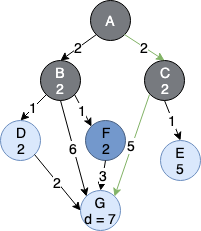
\includegraphics[width=\linewidth]{images/a_star_expansion4.png}
     \caption{Iteration 4}
  \end{subfigure}
  \hfill
  \begin{subfigure}[b]{0.2\linewidth}
    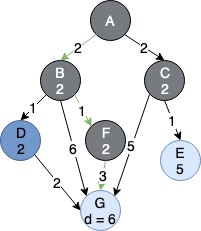
\includegraphics[width=\linewidth]{images/a_star_expansion5.png}
     \caption{Iteration 5}
  \end{subfigure}
  \hfill
  \begin{subfigure}[b]{0.2\linewidth}
    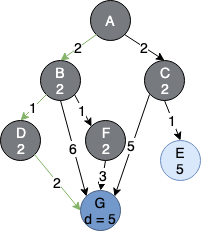
\includegraphics[width=\linewidth]{images/a_star_expansion6.png}
    \caption{Iteration 6}
  \end{subfigure}
  \hfill
  \begin{subfigure}[b]{0.2\linewidth}
    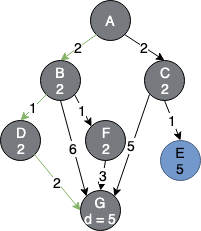
\includegraphics[width=\linewidth]{images/a_star_expansion7.png}
    \caption{Iteration 7}
  \end{subfigure}
  \caption{A* algorithm run on a directed weighted graph. Nodes are labelled with a letter that represents its name (A and G are special nodes agent and goal respectively) and the optimistic heuristic value. Edges have an associated value with them, which represents the actual distance between them. The green node is the goal, dark grey nodes are visited nodes, light blue and dark blue nodes are belonging to the priority queue, dark blue nodes are the next nodes to be expanded, green arrow trace is the optimal solution so far and $d = x$ label is optimal total distance so far}
  \label{fig:a_star_expansion}
\end{figure}

\pagebreak

\begin{algorithm}[h!]
\caption{A*}
\label{alg: a_star}
\begin{algorithmic}[1]

\Procedure{Get-Backtrace}{$p$, $M\colon(A, Os, G)$}
    \State $current \gets$ $G$
    \State $trace \gets [current]$
    \State
    \While {$current$ is not $A$}
        \State $current \gets p[$current$]$
        \State add $current$ to $trace$
    \EndWhile
    \State
    \State \Return reversed $trace$
\EndProcedure
\\

\Procedure{A*}{$M\colon(A, Os, G)$}
    \State Initialize priority queue $pq$ with ($f(A)$, $A$)
    \State $visited \gets \{\}$
    \State $p \gets \{\colon\}$
    \Repeat
        \State $current\_node$ $\gets$ best $n_{best}$ from $pq$ where $\forall n.f(n_{best}) \leq f(n)$
        \State add $current\_node$ to $visited$
        \State
        \If {$current\_node$ is $G$}
            \State follow $\textit{Get-Backtrace}(p, M)$
            \State \Return
        \EndIf
        \State
        \For {\textbf{each} $neighbour$ in $Neighbours(current\_node)$}
            \If {$neighbour$ is not in $visited$ \textbf{or} $g(current\_node) + c(current\_node, neighbour) < g(neighbour)$}
                \State $g(neighbour) \gets g(current\_node) + c(current\_node, neighbour)$
                \State add $neighbour$ to $pq$
                \State update $p[neighbour]$ to $current\_node$
            \EndIf
        \EndFor
    \Until $visited$ is empty
    \State
    \State goal was not found
\EndProcedure
\end{algorithmic}
\end{algorithm}

\subsection{Dijkstra} \label{sec: dijkstra}
The Dijkstra algorithm \cite{choset2005principles, zhang2014multiple} (See Figures \ref{fig:dijkstra}, \ref{fig:dijkstra_expansion}) is a variation of the A* algorithm where we omit the heuristic function ($f(n) = g(n)$). Therefore the algorithm becomes greedy, meaning that we expand the node with lowest distance from the agent position. (See Figure \ref{fig:dijkstra_expansion}). The algorithm is identical to A* (See Algorithm \ref{alg: a_star}), but with $f(n) = g(n)$. Thus, the space and time complexity is the same as A* $(\mathcal{O}(\hat{b}^d))$, but $\hat{b}$ is usually not as efficient as A*.

The major difference between A* and Dijkstra is that, because it is a greedy algorithm, once we expand the goal node, we find the final solution. The solution is optimal in terms of minimal distance because after we expand a node, its distance will not be modified in the future (the invariant holds for all nodes, not only for the goal). 

The drawback of using this method against A* is that it usually explores more than A* and thus the memory gets quite high.

\pagebreak

\begin{figure}[h!]
  \centering
  \begin{subfigure}[b]{0.2\linewidth}
    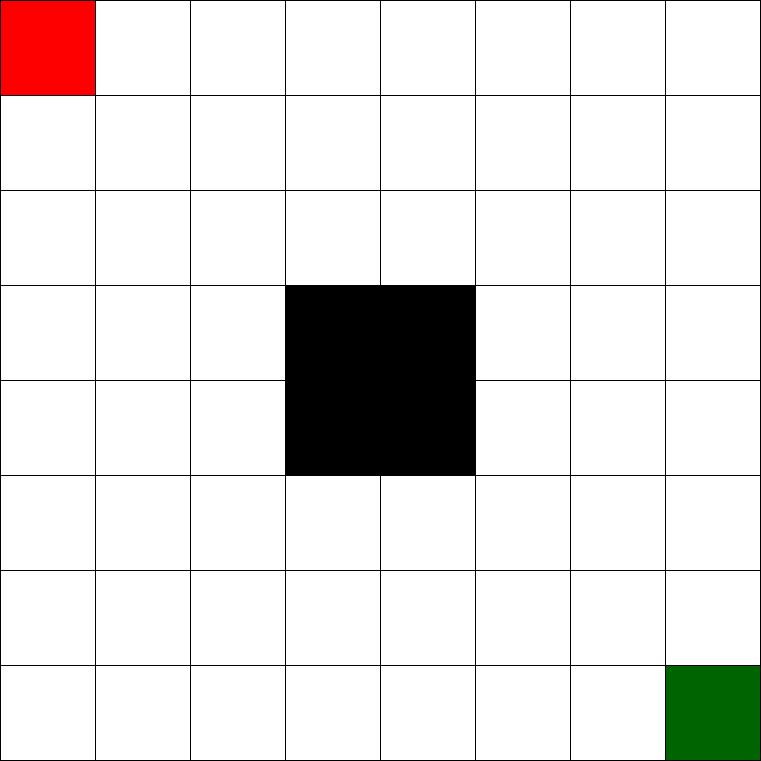
\includegraphics[width=\linewidth]{images/simple_grid.png}
     \caption{Starting 8x8 grid}
  \end{subfigure}
  \hfill
  \begin{subfigure}[b]{0.2\linewidth}
    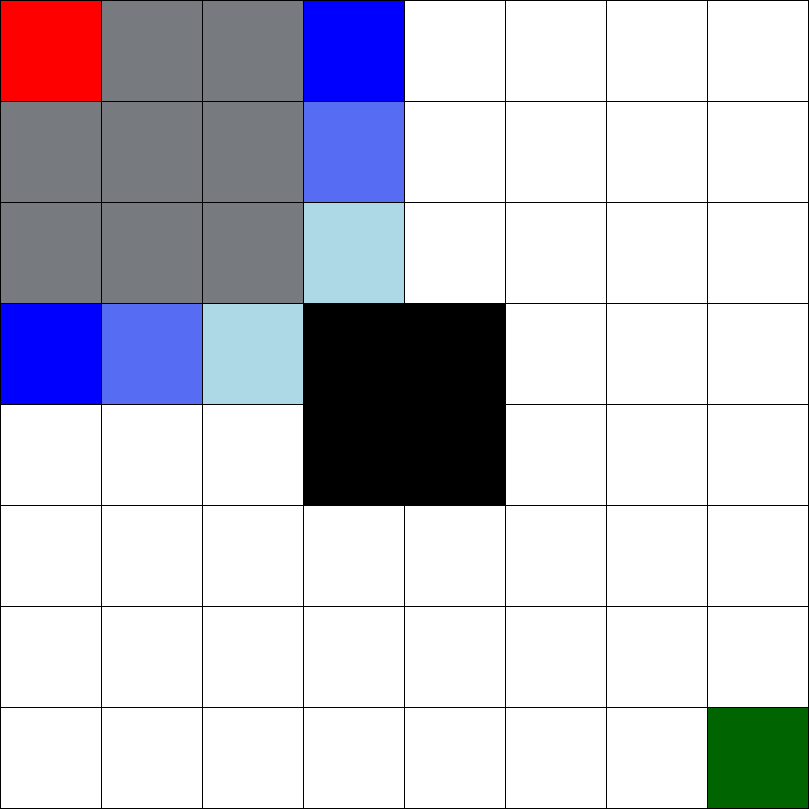
\includegraphics[width=\linewidth]{images/dijkstra1.png}
     \caption{Iteration 1}
  \end{subfigure}
  \hfill
  \begin{subfigure}[b]{0.2\linewidth}
    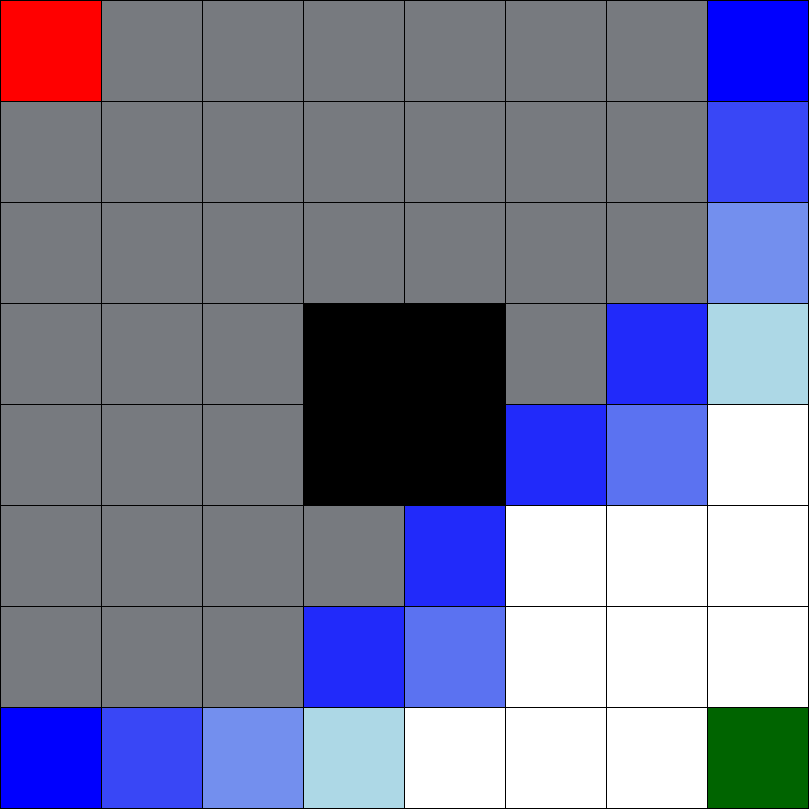
\includegraphics[width=\linewidth]{images/dijkstra2.png}
    \caption{Iteration 2}
  \end{subfigure}
  \hfill
  \begin{subfigure}[b]{0.2\linewidth}
    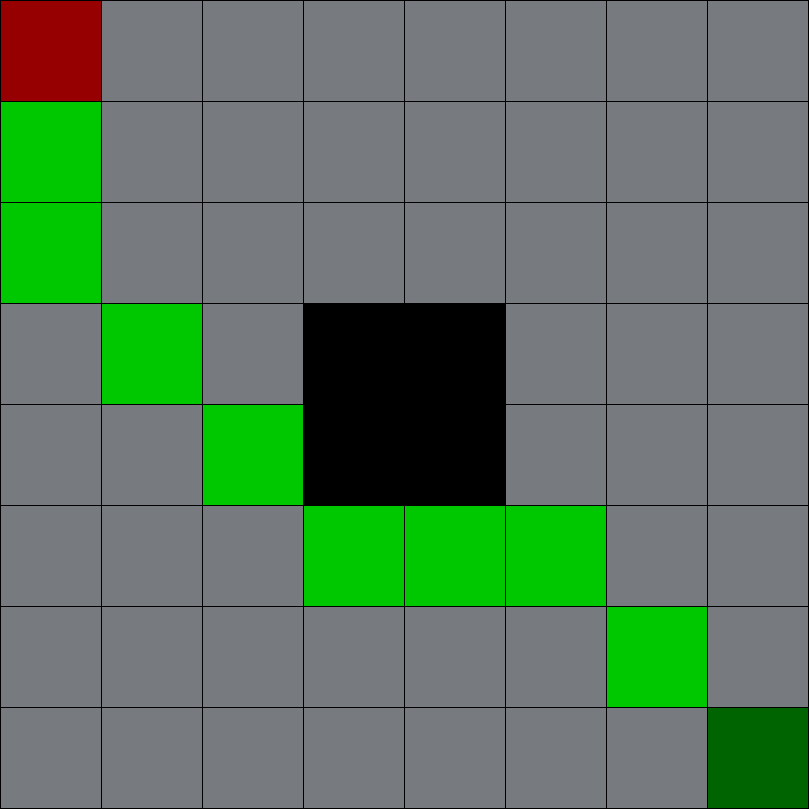
\includegraphics[width=\linewidth]{images/dijkstra3.png}
    \caption{Final trace}
  \end{subfigure}
  \caption{Dijkstra algorithm run on an 8$\times$8 grid (4 iteration points shown: start, 1, 2, final trace). The red square represents the agent start position, the dark green square represents the goal position, black squares represent obstacles, white squares represent the clear path, light green squares represent the final path chosen by the algorithm. The dark grey squares represent the visited set, and the blue squares represent the priority queue (the darker the blue, the higher the priority)}
  \label{fig:dijkstra}
\end{figure}

\begin{figure}[h!]
  \centering
  \begin{subfigure}[b]{0.2\linewidth}
    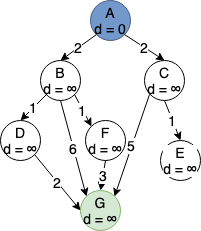
\includegraphics[width=\linewidth]{images/dijkstra_expansion1.png}
     \caption{Iteration 1}
  \end{subfigure}
  \hfill
  \begin{subfigure}[b]{0.2\linewidth}
    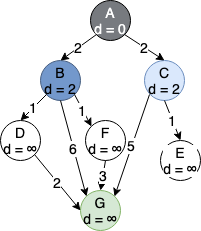
\includegraphics[width=\linewidth]{images/dijkstra_expansion2.png}
     \caption{Iteration 2}
  \end{subfigure}
  \hfill
  \begin{subfigure}[b]{0.2\linewidth}
    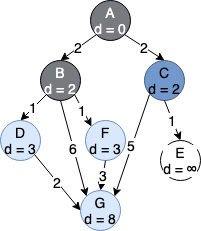
\includegraphics[width=\linewidth]{images/dijkstra_expansion3.png}
    \caption{Iteration 3}
  \end{subfigure}
  \hfill
  \begin{subfigure}[b]{0.2\linewidth}
    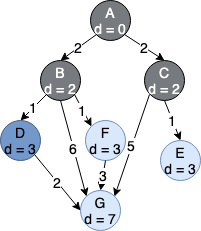
\includegraphics[width=\linewidth]{images/dijkstra_expansion4.png}
     \caption{Iteration 4}
  \end{subfigure}
  \newline
  \begin{subfigure}[b]{0.2\linewidth}
    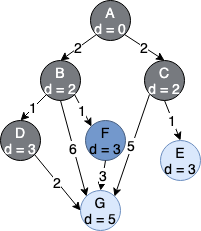
\includegraphics[width=\linewidth]{images/dijkstra_expansion5.png}
     \caption{Iteration 5}
  \end{subfigure}
  \hfill
  \begin{subfigure}[b]{0.2\linewidth}
    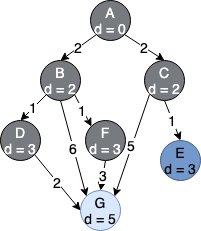
\includegraphics[width=\linewidth]{images/dijkstra_expansion6.png}
    \caption{Iteration 6}
  \end{subfigure}
  \hfill
  \begin{subfigure}[b]{0.2\linewidth}
    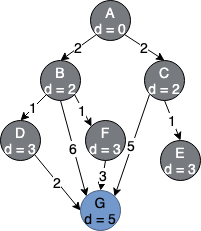
\includegraphics[width=\linewidth]{images/dijkstra_expansion7.png}
     \caption{Iteration 7}
  \end{subfigure}
  \hfill
  \begin{subfigure}[b]{0.2\linewidth}
    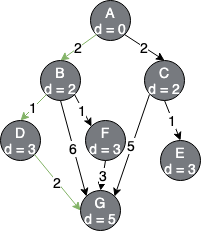
\includegraphics[width=\linewidth]{images/dijkstra_expansion8.png}
    \caption{Iteration 8}
  \end{subfigure}
  \hfill
  \caption{Dijkstra algorithm run on a directed weighted graph. Nodes are labelled with a letter identifier (A and G are special nodes agent and goal respectively) and the current distance. The distance is final when the node is marked as visited. Edges have an associated value with them, which represents edge weight. The green node is the goal, dark grey nodes are visited nodes, light blue and dark blue nodes are belonging to the priority queue, dark blue nodes are the next nodes to be expanded, green arrow trace is the optimal solution}
  \label{fig:dijkstra_expansion}
\end{figure}

\pagebreak

\subsection{Bug Algorithms}
The bug algorithms \cite{choset2005principles, rajko2001pursuit} are one of the earliest and simplest sensor-based solutions for the pathfinding problem, and we will cover two implementations: Bug1 and Bug2. There exist other algorithms which are more advanced such as Tangent Bug described in \cite{choset2005principles, rajko2001pursuit, kamon1998tangentbug}, but we will not cover them as it exceeds the scope of our report.

The idea behind bug algorithms is based on the instinctual behaviour of a bug moving directly towards a destination (goal) and turning around encountered obstacles. The algorithms have two phases: straight line movement (phase 1) and object boundary following (phase 2). We will assume that the agent has a contact sensor that detects if the agent is in the proximity of the boundary of an obstacle.

%We will cover the boundary following algorithm at the end of this section.

The bug algorithms are trivial to implement, not computationally expensive, and it has been shown that their success is guaranteed, meaning that they can find a path to the goal if one exists. However, they do not find the optimal path.

\subsubsection{Bug1} \label{sec: bug1}

First, we label the direction from the agent position to the goal position with $dir_{AG} = \frac{d(A, G)
}{\norm{d(A, G)}} = \frac{(G - A)} {\norm{G - A}}$. In the first phase, the algorithm follows $dir_{A, G}$ until an obstacle is detected and we mark this position as $P_{i}$. Afterwards, it proceeds with the second phase by doing a complete loop around the obstacle while registering the closest distance on the boundary to the goal (find $\hat{Ob} = \argmin{Ob}{d_{Ob, G}}, Ob \in Boundary(O)$) until we reach $P_{i}$. After that, we follow the boundary again until we reach $\hat{Ob}$ and return to the first phase. We repeat this process until the goal is found. If the agent were to move, but it can't from $\hat{Ob}$, then we conclude the algorithm as the goal is unreachable (See Figure \ref{fig:Bug1}, See Algorithm \ref{alg: bug1}) \cite{lumelsky1986dynamic}.

As it is quite hard to estimate the worst case time complexity, we are going to express it as the number of steps upper bound ($\mathcal{O}(upper_{Bug1})$). The upper bound on the number of steps is given by the total distance from the agent to the goal $d(A, G)$, in the case of no obstacles, plus the worst case traversed boundary length for all obstacles $1.5 \sum_{o \in O} length(Boundary(o))$. The space complexity is $\mathcal{O}(1)$ (not counting recursion steps as it can be collapsed in a while loop).

$$upper_{Bug1} = d(A, G) + 1.5 \sum_{o \in O} length(Boundary(o))$$

\begin{figure}[h!]
  \centering
  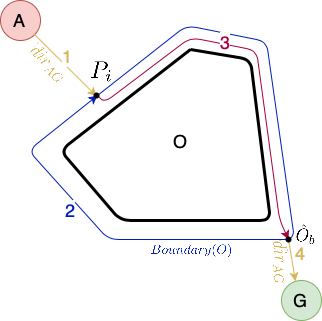
\includegraphics[scale=0.4]{images/Bug1.png}
  \caption{Bug1: Arrows represent the movement direction and numbers represent the traversal order. Yellow arrows represent the first phase. Blue and red arrows represent the second phase}
  \label{fig:Bug1}
\end{figure}

\begin{algorithm}
\caption{Bug1}
\label{alg: bug1}
\begin{algorithmic}[1]
\Procedure{Bug1}{$M\colon(A, Os, G)$}
    \State $\textit{Phase1}(M)$
\EndProcedure
\\
\Procedure{Phase1}{$M\colon(A, Os, G)$}
    \State move agent towards goal along $dir_{A, G}$ until hits $P_i$ or $G$
    \If {$G$ was reached}
        \State \Return
    \EndIf
    \State $\textit{Phase2}(M, P_i)$
\EndProcedure
\\
\Procedure{Phase2}{$M\colon(A, Os, G)$, $P_i$}
    \State find obstacle $O$ with hit point $P_i$ from $Os$
    \State do a full loop around $Boundary(O)$ while computing $\hat{O}b$
    \State follow $Boundary(O)$ until $\hat{O}b$ is reached
    \State
    \If {can't move from $\hat{Ob}$ to $G$}
        \State goal can't be reached
        \State \Return
    \EndIf
    \State
    \State $\textit{Phase1}(M)$
\EndProcedure
\end{algorithmic}
\end{algorithm}

\subsubsection{Bug2} \label{sec: bug2}
The first stage is identical to the one in Bug1, but the second stage follows a greedy approach. Instead of making a full obstacle loop in the second stage, we try to find the point $P \in Boundary(O)$ which belongs to the line segment determined by the original starting agent position and the goal position $P \in LS_{A_{initial}, G}$. $P$ should also be chosen in such a way that it is closer than the original point of contact with the obstacle $P_i$. If $P = P_i$ then the goal can't be reached (See Figure \ref{fig:Bug2}, See Algorithm \ref{alg: bug2}) \cite{lumelsky1986dynamic}.

However, this does not imply that Bug2 outperforms Bug1 in all cases. The time complexity (given as the upper bound) for Bug2 is determined by the total distance from the agent to the goal $d(A, G)$, in the case of no obstacles, plus the worst case traversed boundary length for all obstacles $0.5 \sum_{o \in O} n_{o} \cdot length(Boundary(o))$. The issue here is that, because we follow a greedy approach, we might reencounter the same obstacle, thus $n_{o}$ represents how many times we have encountered obstacle $o$. Therefore, Bug1 might yield better performance in cases where the environment contains complex obstacles. The space complexity is still $\mathcal{O}(1)$.

$$upper_{Bug2} = d(A, G) + 0.5 \sum_{o \in O} n_{o} \cdot length(Boundary(o))$$

\begin{figure}[h!]
  \centering
  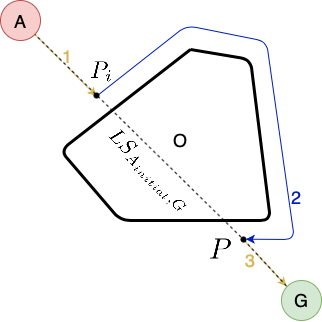
\includegraphics[scale=0.4]{images/Bug2.png}
  
  \caption{Bug2: Arrows represent the movement direction and numbers represent the traversal order. Yellow arrows represent the first phase. Blue arrows represent the second phase}
  \label{fig:Bug2}
\end{figure}

\begin{algorithm}[h]
\caption{Bug2}
\label{alg: bug2}
\begin{algorithmic}[1]
\Procedure{Bug2}{$M\colon(A, Os, G)$}
    \State $\textit{Phase1}()$
\EndProcedure
\\
\Procedure{Phase1}{$M\colon(A, Os, G)$}
    \State move agent towards goal along $LS_{A_{initial}, G}$ until hits $P_i$ or $G$
    \If {$G$ was reached}
        \State \Return
    \EndIf
    \State $\textit{Phase2}(M, P_i)$
\EndProcedure
\\
\Procedure{Phase2}{$M\colon(A, Os, G)$, $P_i$}
    \State find obstacle $O$ with hit point $P_i$ from $Os$
    \State follow $Boundary(O)$ until we hit $P \in LS_{A_{initial}, G}$, $d(P_{i}, G) \geq d(P, G)$
    \State
    \If {$P$ = $P_i$}
        \State goal can't be reached
        \State \Return
    \EndIf
    \State
    \State $\textit{Phase1}(M)$
\EndProcedure
\end{algorithmic}
\end{algorithm}

%\textbf{Tangent Bug}

%\textbf{Curve Tracing}

\subsection{Value Iteration on Markovian Decision Processes (MDP)} \label{sec:vin}
The Markovian Decision Process (MDP) \cite{szepesvari2010algorithms, satia1973markovian} (See Figure \ref{fig:MDPWorld}) represents a state environment in which an agent can transition from one state to the next one until it reaches a terminating state. Whenever the agent chooses an action by moving from a state to another, it is rewarded based on the type of action that it took and the previous and next states. 

Formally, a Markovian Decision Process is a tuple $\langle\mathcal{S}, \mathcal{A}, \mathcal{P}_{s, s'}^a, \mathcal{R}_{s, s'}^a, \gamma \in [0, 1], \pi \rangle$. $\mathcal{S}$ is the state space, $\mathcal{A}$ is the action space (what actions are available to the agent), $\mathcal{P}_{s, s'}^a$ is the probability transition matrix which gives the probability of transitioning with action $a$ from state $s$ to state $s'$, $\mathcal{R}_{s, s'}^a$ is the reward matrix and states the reward for taking action $a$ from state $s$ to state $s'$, $\gamma$ is the discounted rewards factor and $\pi$ is the policy which can be deterministic or stochastic.

\begin{figure}[h!]
  \centering
  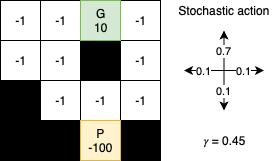
\includegraphics[scale=0.5]{images/MDPWorld.png}
  \caption{An example of an MDP world. White squares represent possible states. The agent can start from \textbf{any} of the white squares. There are 2 special terminal states: the green square represents the goal, and the yellow square represents the penalty state. Each state has an associated reward value which is collected whenever the agent leaves the state (for the terminal states, the reward is collected instantaneously). There are 4 possible actions (up, right, down, left; 4-point connectivity), but each action is stochastic meaning that if the agent chooses a specific direction it will move in that direction with 0.7 probability or it will move to the other directions with equal probability}
  \label{fig:MDPWorld}
\end{figure}

$R_t$ represents the total discounted reward from time step $t$, and it is defined in terms of the collected rewards $r_t$.

$$R_t = r_{t+1} + \gamma r_{t + 2} + \gamma^2 r_{t + 3} + ... = \sum_{k = 0}^{\infty} \gamma^k r_{t + k + 1}$$

The value function $V^{\pi}(s)$, where $\pi$ is the policy,  with signature $V^{\pi} \colon \mathcal{S} \xrightarrow{} \mathbb{R}$ represents a method for assessing how "good" a state is. It is defined as the expected total discounted reward.

$$V^{\pi}(s) = \mathbb{E}_{\pi}[R_t|S_t = s] = \sum_{a \in \mathcal{A}} \pi(s, a) \sum_{s' \in S} \mathcal{P}_{s, s'}^a (\mathcal{R}_{s, s'}^a + \gamma V^{\pi}(s'))$$

The state-action value function $Q^{\pi}(s, a)$ with signature $Q^{\pi} \colon \{ \mathcal{S}, \mathcal{A} \} \xrightarrow{} \mathbb{R}$ represents a method for assessing how "good" a state is, given a certain action.

$$Q^{\pi}(s, a) = \mathbb{E}_{\pi}[R_t|S_t = s, A_t = a] = \sum_{s' \in S} \mathcal{P}_{s, s'}^a (\mathcal{R}_{s, s'}^a + \gamma V^{\pi}(s'))$$

This also means that we can define $V^{\pi}(s)$ in terms of $Q^{\pi}(s, a)$.

$$V^{\pi}(s) = \sum_{a \in \mathcal{A}} \pi(s, a) Q^{\pi}(s, a)$$

\begin{Theo}{Bellman Optimality Equation}{Bellman}
The Bellman Optimality Equation states that the optimal value function is given by the following formula:
\begin{align*}
    V^{\pi^{*}}(s) &= \max_{a} \sum_{s' \in S} \mathcal{P}_{s, s'}^a (\mathcal{R}_{s, s'}^a + \gamma V^{\pi^{*}}(s')) = \max_{a} Q^{\pi^{*}}(s, a)\\
    Q^{\pi^{*}}(s, a) &= \sum_{s' \in S} \mathcal{P}_{s, s'}^a (\mathcal{R}_{s, s'}^a + \gamma V^{\pi^{*}}(s'))
\end{align*}
\end{Theo}

By following the Bellman Optimality Equation (\Cref{Th:Bellman}), we can devise a dynamic programming algorithm called Value Iteration. The algorithm updates $\mathcal{V^{\pi}}$ in place by applying the Bellman Optimality Equation for each state, thus finding better $\mathcal{V^{\pi}}$ on each run. We repeat the process until we see no further changes in $\mathcal{V^{\pi}}$. This means that $\mathcal{V^{\pi}}$ has converged for all $s \in \mathcal{S}$. After that, we return the optimal policy by choosing the optimal action at each state $s \in \mathcal{S}$ (See Algorithm \ref{alg: value_iteration}). If we run the algorithm on the MDP world defined in Figure \ref{fig:MDPWorld}, we will get the results presented in Figure \ref{fig:MDPResults}.

\begin{figure}[h!]
  \centering
  \begin{subfigure}[b]{0.3\linewidth}
    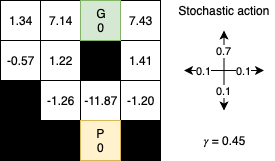
\includegraphics[width=\linewidth]{images/MDPWorldResult.png}
     \caption{Optimal value function}
  \end{subfigure}
  \hspace{1.3cm}
  \begin{subfigure}[b]{0.3\linewidth}
    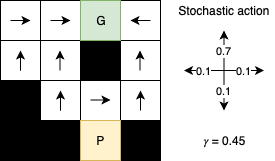
\includegraphics[width=\linewidth]{images/MDPWorldResultPolicy.png}
     \caption{Optimal policy}
  \end{subfigure}
  \caption{The results after applying the Value Iteration algorithm on the MDP World defined in figure \ref{fig:MDPWorld}. On the left, each cell contains the optimal value function $V^{\pi}(s)$. The optimal policy is displayed on the right}
  \label{fig:MDPResults}
\end{figure}

\begin{algorithm}
\caption{Value Iteration}
\label{alg: value_iteration}
\begin{algorithmic}[1]
\Procedure{Value-Iteration}{$\mathcal{S}$, $\mathcal{A}$, $\mathcal{P}$, $\mathcal{R}, \gamma$}
    \State Initialize $\mathcal{V^{\pi}}$, $\pi$ arbitrarily (e.g. all 0)
    \State
    \Repeat
        \For {\textbf{each} $s \in \mathcal{S}$}
            \State $V^{\pi}(s) = \underset{a \in \mathcal{A}}{\max} \hspace{0.1cm} \sum_{s' \in S} \mathcal{P}_{s, s'}^a (\mathcal{R}_{s, s'}^a + \gamma V^{\pi}(s'))$
        \EndFor
    \Until we have no change in $\mathcal{V^{\pi}}$
    \State
    
    \For {\textbf{each} $s \in \mathcal{S}$}
        \State $\pi(s) = \argmax{a \in \mathcal{A}}{\sum_{s' \in S} \mathcal{P}_{s, s'}^a (\mathcal{R}_{s, s'}^a + \gamma V^{\pi}(s'))}$
    \EndFor
    \State \textbf{return} $\pi$
\EndProcedure
\end{algorithmic}
\end{algorithm}

The time complexity is $\mathcal{O}(c|S||\mathcal{A}|)$ and the space complexity is $\mathcal{O}(|S|)$, where $c$ is the convergence rate, $|S|$ is the number of states and $|\mathcal{A}|$ is the number of actions. The time complexity is given by the update rule (which is $\mathcal{O}(|S||\mathcal{A}|)$, for each state we find the maximising action) being run $c$ times (some notebooks state that $c$ is bounded by $|S|$) and the final policy evaluation (which is still $\mathcal{O}(|S||\mathcal{A}|)$). The space complexity is given by the number of elements in $\mathcal{V^{\pi}}$ and $\pi$, which is the number of states $|S|$.

The advantage of using MDPs is that we can model a more complex world for the agent in which we can define areas which should be avoided (such as bridges, because they draw more battery power) by associating a negative reward with them. However, it can also be considered a disadvantage for worlds that cannot be easily modelled, as we have to know the transition probabilities and rewards apriori before we can apply Value Iteration. Not to mention that the number of states can get quite big. For instance, let us assume that we have a robotic arm with 3 joints, and each join can rotate 180\degree. If we discretise each angle into 1\degree angles, we will have a total number of $180^3 \simeq 5.8$ million states. There exist algorithms which can handle a large number of states such as Monte Carlo (sampling episode traces) and Temporal Difference Learning (combines dynamic programming and sampling), but we will not cover them as they are out of the report's scope \cite{szepesvari2010algorithms}.
